% This is a template file for Sweave used in MAGeCK
% Author: Wei Li, Shirley Liu lab
% Do not modify lines beginning with "#__".
\documentclass{article}

\usepackage{amsmath}
\usepackage{amscd}
\usepackage[tableposition=top]{caption}
\usepackage{ifthen}
\usepackage{fullpage}
\usepackage[utf8]{inputenc}

\usepackage{Sweave}
\begin{document}
\Sconcordance{concordance:defaultTest_defaultNormCount_screen1_summary.tex:defaultTest_defaultNormCount_screen1_summary.Rnw:%
1 12 1 1 0 14 1 1 8 2 1 1 14 12 0 1 6 12 0 1 6 12 0 1 2 24 1 1 4 2 1 1 %
99 1 13 6 1 1 140 1 2 2 1 1 140 1 2 2 1 1 72 1 2 4 1 1 4 2 1 1 99 1 13 %
6 1 1 140 1 2 2 1 1 140 1 2 2 1 1 72 1 2 11 1}

\setkeys{Gin}{width=0.9\textwidth}

\title{MAGeCK Comparison Report}
\author{Wei Li}

\maketitle


\tableofcontents

\section{Summary}

%Function definition

The statistics of comparisons is as indicated in the following table. 

% latex table generated in R 4.0.0 by xtable 1.8-4 package
% Thu Jun 25 16:12:02 2020
\begin{table}[ht]
\centering
\begin{tabular}{rlrlrrr}
  \hline
 & Comparison & Genes & Selection & FDR1\% & FDR5\% & FDR10\% \\ 
  \hline
1 & FXN High Gate vs Baseline & 19280 & positive & 32 & 183 & 419 \\ 
   \hline
\end{tabular}
\caption{Number of genes detected as significantly enriched in FXN High samples} 
\label{tab:one}
\end{table}% latex table generated in R 4.0.0 by xtable 1.8-4 package
% Thu Jun 25 16:12:02 2020
\begin{table}[ht]
\centering
\begin{tabular}{rlrlrrr}
  \hline
 & Comparison & Genes & Selection & FDR1\% & FDR5\% & FDR10\% \\ 
  \hline
1 & FXN High Gate vs Baseline & 19280 & positive & 32 & 183 & 419 \\ 
   \hline
\end{tabular}
\caption{Number of genes detected as significantly enriched in FXN High samples} 
\label{tab:one}
\end{table}% latex table generated in R 4.0.0 by xtable 1.8-4 package
% Thu Jun 25 16:12:02 2020
\begin{table}[ht]
\centering
\begin{tabular}{rlrlrrr}
  \hline
 & Comparison & Genes & Selection & FDR1\% & FDR5\% & FDR10\% \\ 
  \hline
1 & FXN High Gate vs Baseline & 19280 & positive & 32 & 183 & 419 \\ 
   \hline
\end{tabular}
\caption{Number of genes detected as significantly enriched in FXN High samples} 
\label{tab:one}
\end{table}
The meanings of the columns are as follows.

\begin{itemize}
\item \textbf{Comparison}: The label for comparisons;
\item \textbf{Genes}: The number of genes in the library;
\item \textbf{Selection}: The direction of selection, either positive selection or negative selection;
\item \textbf{FDR1\%}: The number of genes with FDR $<$ 1\%;
\item \textbf{FDR5\%}: The number of genes with FDR $<$ 5\%;
\item \textbf{FDR25\%}: The number of genes with FDR $<$ 25\%;
\end{itemize}

The following figures show:

\begin{itemize}
\item Individual sgRNA read counts of selected genes in selected samples; 
\item The distribution of RRA scores and p values of all genes; and
\item The RRA scores and p values of selected genes.
\end{itemize}


\newpage\section{Comparison results of fxn 1 vs rest neg.}

The following figure shows the distribution of RRA score in the comparison fxn 1 vs rest neg., and the RRA scores of 10 genes.

%


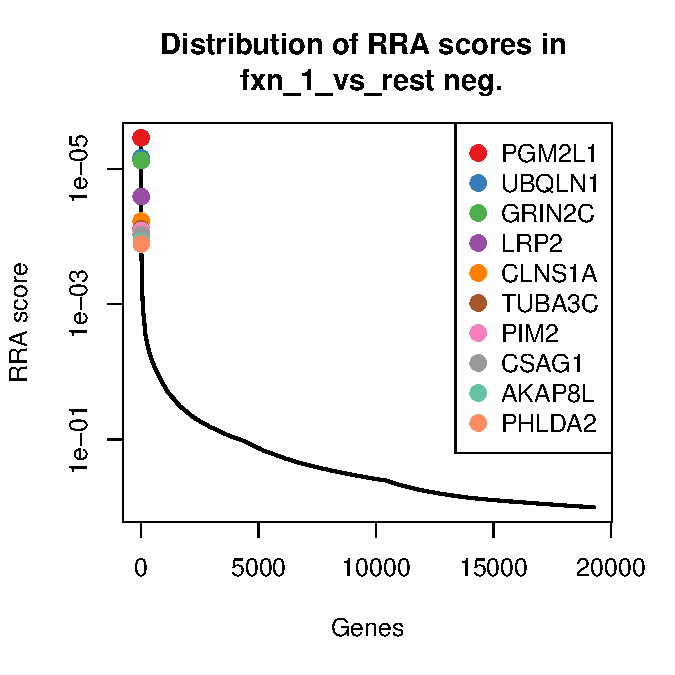
\includegraphics{defaultTest_defaultNormCount_screen1_summary-004}
%%
\clearpage
\newpage
The following figures show the distribution of sgRNA read counts (normalized) of selected genes in selected samples.
%


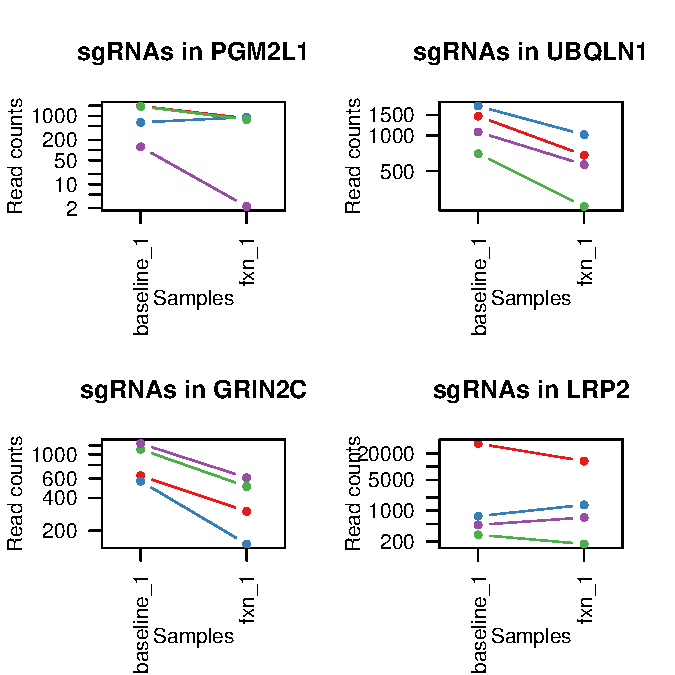
\includegraphics{defaultTest_defaultNormCount_screen1_summary-005}
%


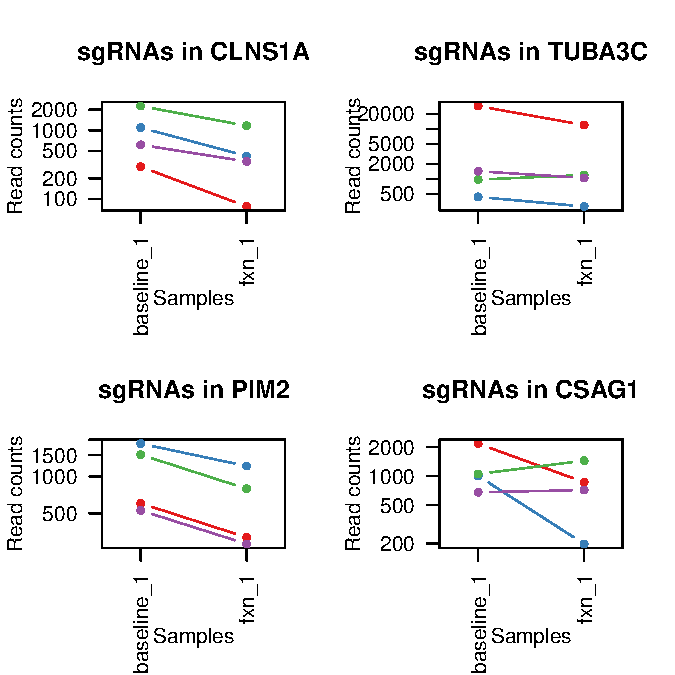
\includegraphics{defaultTest_defaultNormCount_screen1_summary-006}
%


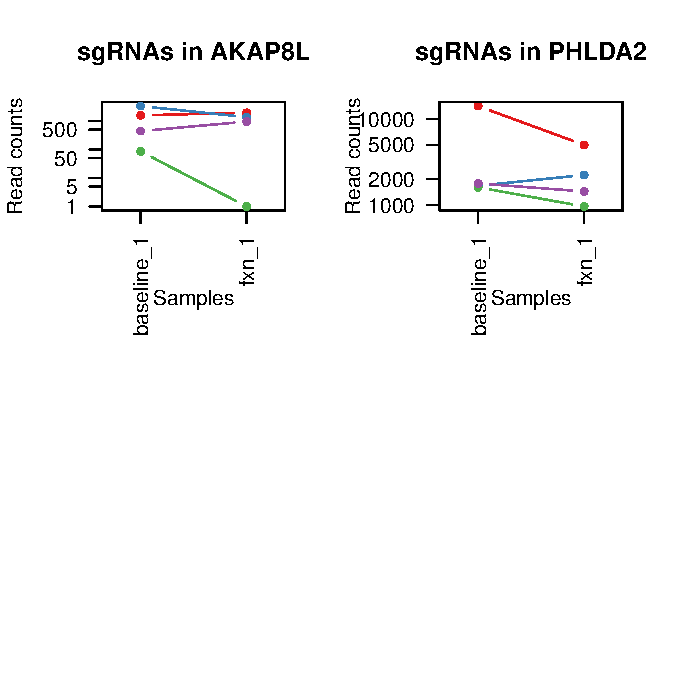
\includegraphics{defaultTest_defaultNormCount_screen1_summary-007}

\newpage\section{Comparison results of fxn 1 vs rest pos.}

The following figure shows the distribution of RRA score in the comparison fxn 1 vs rest pos., and the RRA scores of 10 genes.

%


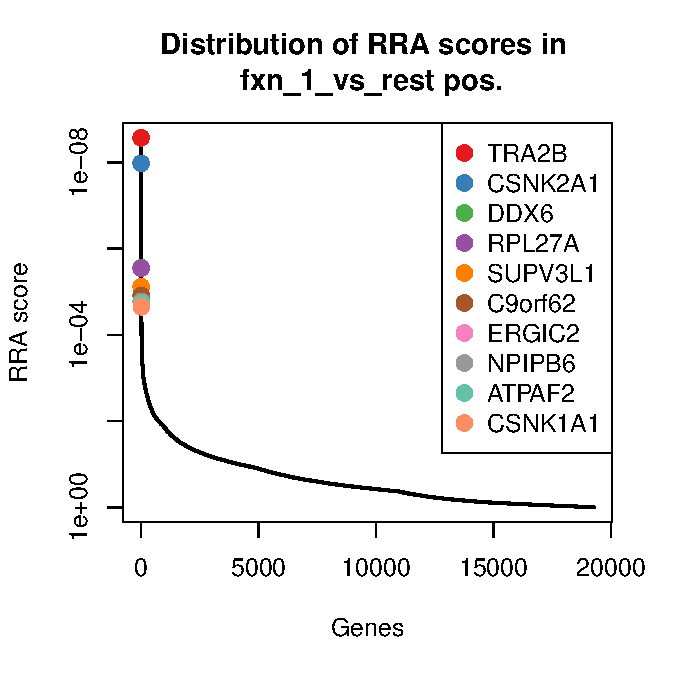
\includegraphics{defaultTest_defaultNormCount_screen1_summary-009}
%%
\clearpage
\newpage
The following figures show the distribution of sgRNA read counts (normalized) of selected genes in selected samples.
%


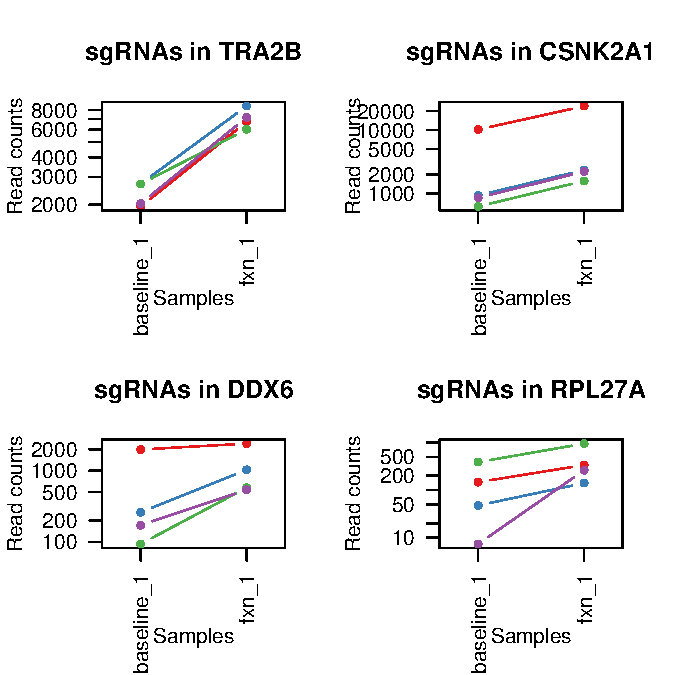
\includegraphics{defaultTest_defaultNormCount_screen1_summary-010}
%


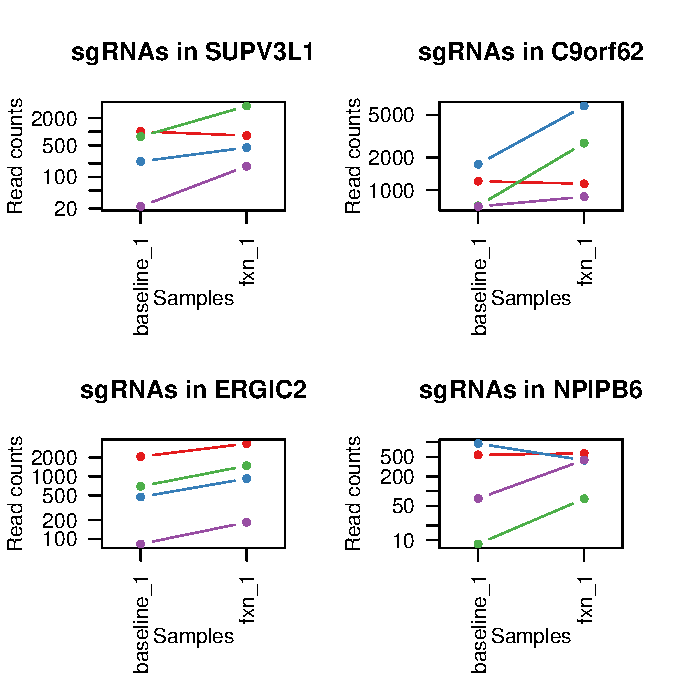
\includegraphics{defaultTest_defaultNormCount_screen1_summary-011}
%


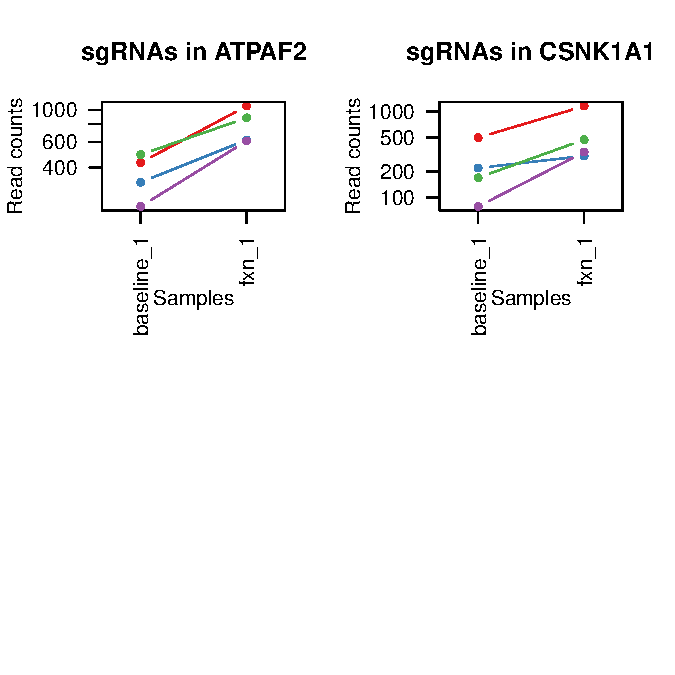
\includegraphics{defaultTest_defaultNormCount_screen1_summary-012}
%__INDIVIDUAL_PAGE__









\end{document}

